% SC4002 --- Chapter 5: Language Models --- Smoothing and Neural LMs (0->100 ground-up)
% No \documentclass --- \included by modules/SC4002/main.tex (book class).
\chapter{Language Models: Smoothing and Neural Prediction}\label{ch:language-model}
\begin{quote}
\emph{``A language model is an imagination trained on counting: given what came before, what comes next?''} --- This chapter turns that question from raw counts into smoothed probabilities and then into neural networks.
\end{quote}
\noindent\fbox{\parbox{\dimexpr\linewidth-2\fboxsep-2\fboxrule}{%
\textbf{From zero: no LM background assumed.} We start from the everyday idea of autocompleting a sentence, ask why counting $n$-grams always leaves gaps, and fix those gaps by smoothing. Then we replace tables of counts with a network that predicts the next word and measure it with perplexity. Every formula is motivated by a picture first.}}
\vspace{0.3em}
\section*{Learning Outcomes}
After this chapter you will be able to:
\begin{enumerate}[label=(L\arabic*)]
    \item explain the chain rule and the Markov assumption for $n$-gram models;
    \item write the MLE and explain why sparsity forces smoothing;
    \item compare Laplace, Good--Turing, and interpolated Kneser--Ney smoothing;
    \item describe feedforward and RNN neural LMs (softmax + cross-entropy);
    \item define perplexity as $2^{H}$ and use it to compare models.
\end{enumerate}
% ============================================================
\section{Predicting the Next Word: Why Counting Is Not Enough}\label{sec:next-word}
\paragraph{Intuition.} Type ``the cat sat on the'' into your phone. It suggests ``mat'' before you finish. A \textbf{language model} (LM) assigns a probability $P(w_{1}^{m})$ to any word sequence, or equivalently $P(w_{i}\mid w_{1}^{i-1})$ to the next word given history. By the chain rule
\begin{equation}
P(w_{1}^{m})=\prod_{i=1}^{m} P(w_{i}\mid w_{1}^{i-1}), \quad w_{i}\in\mathcal{V}.
\label{eq:chain}
\end{equation}
An $n$-gram makes a $(n-1)$-th order Markov assumption: keep only the last $n-1$ words, e.g.\ $P(w_{i}\mid w_{i-2},w_{i-1})$ for $n=3$. The table is finite, so it can be learned by counting.
\paragraph{Formal: MLE.} Let $c(\cdot)$ be corpus counts. The maximum-likelihood estimate is the count ratio
\begin{equation}
P_{\text{MLE}}(w_{i}\mid w_{i-n+1}^{i-1})=\frac{c(w_{i-n+1}^{i})}{c(w_{i-n+1}^{i-1})},\quad
P_{\text{MLE}}(w_{i}\mid w_{i-1})=\frac{c(w_{i-1},w_{i})}{c(w_{i-1})}.
\label{eq:mle-ngram}
\end{equation}
Example: corpus = ``\texttt{the cat sat}'', ``\texttt{the cat ran}''. Then $P_{\text{MLE}}(\text{sat}\mid\text{cat})=1/2$, $P_{\text{MLE}}(\text{mat}\mid\text{cat})=0/2=0$.
\paragraph{The sparsity problem.} With $|\mathcal{V}|=50\,000$, there are $2.5$B possible bigrams; any corpus sees a tiny fraction. An MLE of $0$ zeroes the whole sentence probability via Eq.~\eqref{eq:chain}: one unseen $n$-gram kills the product. Worse, Zipf's long tail guarantees most $n$-grams are unseen at test time. \textbf{Smoothing} redistributes a little probability from seen to unseen events so no $n$-gram ever gets exactly $0$.
% ============================================================
\section{Smoothing: From Laplace to Kneser--Ney}\label{sec:smoothing}
\paragraph{Laplace (add-$\alpha$) smoothing.} The simplest fix: pretend every $n$-gram occurred $\alpha$ times more. For bigrams with vocabulary size $V$,
\begin{equation}
P_{\text{Lap}}(w_{i}\mid w_{i-1})=\frac{c(w_{i-1},w_{i})+\alpha}{c(w_{i-1})+\alpha V},\quad \alpha=1\text{ is add-one.}
\label{eq:laplace}
\end{equation}
Intuition: we smooth by pulling every estimate toward the uniform $1/V$. Cheap but blunt---it steals too much from frequent $n$-grams when $V$ is large. With $V=50\,000$, add-one adds $50\,000$ phantom counts per history.
\paragraph{Good--Turing: let the counts tell us.} Count how many $n$-grams occurred $r$ times: $N_{r}=|\{n\text{-gram}:c=r\}|$. Good--Turing re-estimates count $r$ as
\begin{equation}
r^{*}=(r+1)\frac{N_{r+1}}{N_{r}},\quad P_{\text{GT}}(w_{i-n+1}^{i})=\frac{r^{*}}{N},\; N=\sum_{r}rN_{r}.
\label{eq:good-turing}
\end{equation}
Events seen once ($r=1$) are discounted using the number seen twice ($N_{2}$); unseen events ($r=0$) get mass $N_{1}/N$ in total---the proportion of singletons. Intuition: the frequency of rare events predicts the chance of unseen ones. Good--Turing is much better for unigrams but not conditional $P(w_{i}\mid\text{history})$ directly.
\paragraph{Kneser--Ney: the right backoff.} Consider ``San Francisco is ...''. Bigram ``San Francisco'' is frequent, but ``Francisco'' occurs almost only after ``San''. If we back off to unigram $P(\text{Francisco})$, it looks common---wrong. Kneser--Ney uses \textbf{continuation probability}: how many \emph{different} contexts does a word follow?
\begin{equation}
P_{\text{cont}}(w)=\frac{|\{v: c(v,w)>0\}|}{|\{(u,v):c(u,v)>0\}|}.
\label{eq:cont}
\end{equation}
``Francisco'' has continuation $1/V$ (only ``San'' precedes it), ``the'' has high continuation. Interpolated Kneser--Ney for bigrams:
\begin{equation}
P_{\text{KN}}(w_{i}\mid w_{i-1})=\frac{\max(c(w_{i-1},w_{i})-D,0)}{c(w_{i-1})}+\lambda(w_{i-1})\,P_{\text{cont}}(w_{i}),
\label{eq:kn}
\end{equation}
where $0<D<1$ is a discount (typically $0.75$) and
\begin{equation}
\lambda(w_{i-1})=\frac{D}{c(w_{i-1})}\,|\{w:c(w_{i-1},w)>0\}|
\label{eq:lambda}
\end{equation}
is the leftover mass given to the backoff. For trigrams it recurses: $P_{\text{KN}}(w_{i}\mid w_{i-2},w_{i-1})$ backs off to bigrams, which back off to $P_{\text{cont}}$. This is the $n$-gram gold standard before neural models.
\begin{figure}[h]
\centering
\begin{tikzpicture}[font=\footnotesize, >=Stealth]
  % raw distribution
  \begin{scope}
    \node[font=\bfseries\scriptsize] at (2.2,3.8) {MLE: spiky + zeros};
    \draw[->] (0,0) -- (4.6,0) node[right, font=\scriptsize] {$w$};
    \draw[->] (0,0) -- (0,3.4) node[above, font=\scriptsize] {$P$};
    \fill[blue!55, draw=blue!60!black] (0.35,0) rectangle (0.75,2.8) node[midway, above, font=\tiny, yshift=1.15cm] {sat};
    \fill[blue!55, draw=blue!60!black] (1.05,0) rectangle (1.45,1.9) node[midway, above, font=\tiny, yshift=0.7cm] {ran};
    \fill[blue!15, draw=blue!40!black] (1.75,0) rectangle (2.15,0.05);
    \fill[blue!15, draw=blue!40!black] (2.45,0) rectangle (2.85,0.05);
    \fill[blue!15, draw=blue!40!black] (3.15,0) rectangle (3.55,0.05);
    \fill[blue!15, draw=blue!40!black] (3.85,0) rectangle (4.25,0.05);
    \node[font=\tiny, fill=red!10, draw=red!40!black, rounded corners=2pt, inner sep=2pt] at (3.05,2.2) {many $=0$};
    \draw[->, red!60!black, thick, dashed] (3.05,1.85) -- (3.5,0.3);
    \node[font=\tiny, text=gray!60!black] at (2.2,-0.6) {history = ``cat''};
  \end{scope}
  \begin{scope}[xshift=6.2cm]
    \node[font=\bfseries\scriptsize] at (2.2,3.8) {Smoothed: everyone gets $>0$};
    \draw[->] (0,0) -- (4.6,0) node[right, font=\scriptsize] {$w$};
    \draw[->] (0,0) -- (0,3.4) node[above, font=\scriptsize] {$P$};
    \fill[orange!45, draw=orange!60!black] (0.35,0) rectangle (0.75,2.35);
    \fill[orange!45, draw=orange!60!black] (1.05,0) rectangle (1.45,1.65);
    \fill[orange!30, draw=orange!60!black] (1.75,0) rectangle (2.15,0.55) node[midway, above, font=\tiny, yshift=0.2cm] {mat};
    \fill[orange!30, draw=orange!60!black] (2.45,0) rectangle (2.85,0.50);
    \fill[green!25, draw=green!55!black] (3.15,0) rectangle (3.55,0.40);
    \fill[green!25, draw=green!55!black] (3.85,0) rectangle (4.25,0.40);
    \node[font=\tiny, fill=green!10, draw=green!50!black, rounded corners=2pt, inner sep=2pt] at (2.95,2.9) {discounted};
    \node[font=\tiny, fill=orange!10, draw=orange!50!black, rounded corners=2pt, inner sep=2pt] at (2.95,2.35) {unseen $>0$};
    \draw[->, violet!60!black, thick] (0.55,2.55) -- (0.55,2.80);
    \draw[->, violet!60!black, thick] (1.95,0.55) -- (1.95,0.95);
    \node[font=\tiny, text=gray!60!black] at (2.2,-0.6) {history = ``cat''};
  \end{scope}
  \node[font=\tiny, fill=yellow!10, draw=gray!40, rounded corners=2pt, inner sep=3pt] at (5.4,-1.4) {\textcolor{blue!60!black}{$\blacksquare$ raw MLE} \ \textcolor{orange!60!black}{$\blacksquare$ smoothed} \ \textcolor{green!50!black}{$\blacksquare$ Kneser--Ney cont.}};
\end{tikzpicture}
\caption{Left: MLE leaves most words at exactly zero (red), so any sentence with an unseen continuation gets probability $0$. Right: smoothing discounts seen bars (violet arrow down) and lifts unseen bars above zero (violet arrow up). Kneser--Ney further reweights by continuation counts (green).}
\label{fig:smoothing-bars}
\end{figure}
% ============================================================
\section{Neural Language Models and Perplexity}\label{sec:neural-lm}
\paragraph{Feedforward NNLM (Bengio 2003).} Instead of a table $P(w_{i}\mid w_{i-n+1}^{i-1})$, learn a network. Fix window $n$ (e.g.\ $n=3$). Map each context word to an embedding $\mathbf{e}=\mathbf{E}\mathbf{x}\in\mathbb{R}^{d}$, concatenate, and pass through a hidden layer:
\begin{equation}
\mathbf{h}=\tanh\!\big(\mathbf{W}[\mathbf{e}_{i-n+1};\dots;\mathbf{e}_{i-1}]+\mathbf{b}\big),\quad
\mathbf{z}=\mathbf{U}\mathbf{h}+\mathbf{c}\in\mathbb{R}^{V},\quad
P(w_{i}=v\mid\text{ctx})=\text{softmax}(\mathbf{z})_{v}=\frac{e^{z_{v}}}{\sum_{k=1}^{V}e^{z_{k}}}.
\label{eq:nnlm}
\end{equation}
Training minimizes cross-entropy (negative log-likelihood) over the corpus of length $T$:
\begin{equation}
\mathcal{L}=-\frac1T\sum_{i=1}^{T}\log P(w_{i}\mid w_{i-n+1}^{i-1}),\quad
\nabla_{\mathbf{z}}\mathcal{L}= \mathbf{p}-\mathbf{y}_{\text{one-hot}}.
\label{eq:ce}
\end{equation}
Similar words get similar embeddings, so ``cat sat'' and ``dog sat'' share statistics---a cure for sparsity that no count model achieves. The price is a fixed window.
\paragraph{RNN language model.} Drop the window. An RNN keeps a hidden state that summarizes \emph{all} prior words:
\begin{equation}
\mathbf{h}_{t}=\tanh(\mathbf{W}_{xh}\mathbf{e}_{t}+\mathbf{W}_{hh}\mathbf{h}_{t-1}+\mathbf{b}_{h}),\quad
\mathbf{z}_{t}=\mathbf{W}_{hy}\mathbf{h}_{t}+\mathbf{b}_{y},\quad
P(w_{t+1}\mid w_{1}^{t})=\text{softmax}(\mathbf{z}_{t}).
\label{eq:rnn-lm}
\end{equation}
One matrix $\mathbf{W}_{hh}$ is reused every step (weight tying through time). Training via backpropagation through time (BPTT) unfolds the recurrence. In practice we use LSTM/GRU gates to keep gradients alive. RNNs have unbounded context in principle; Transformers later make that context fully parallel.
\begin{figure}[h]
\centering
\begin{tikzpicture}[
  emb/.style={rectangle, draw=teal!60!black, thick, fill=teal!15, minimum width=1.2cm, minimum height=0.6cm, font=\scriptsize, rounded corners=2pt},
  hid/.style={circle, draw=blue!60!black, thick, fill=blue!15, minimum size=9mm, font=\scriptsize},
  outbox/.style={rectangle, draw=violet!60!black, thick, fill=violet!12, minimum width=1.2cm, minimum height=0.6cm, font=\scriptsize, rounded corners=2pt},
  arr/.style={-{Latex[length=2mm]}, thick, color=gray!70!black}
]
\node[emb] (e1) at (0,0) {$\mathbf{e}_{i-2}$}; \node[emb] (e2) at (1.8,0) {$\mathbf{e}_{i-1}$}; \node[emb] (e3) at (3.6,0) {$\dots$};
\node[font=\tiny, color=teal!60!black] at (1.8,-0.6) {lookup $\mathbf{E}$};
\node[rectangle, draw=orange!60!black, thick, fill=orange!14, minimum width=3.6cm, minimum height=0.65cm, font=\scriptsize, rounded corners=3pt] (concat) at (1.8,1.15) {concat $[\mathbf{e}_{i-n+1};\dots]$};
\foreach \i in {1,2} \draw[arr, color=teal!60!black] (e\i.north) -- (concat.south);
\draw[arr, color=teal!40!black, dashed] (e3.north) -- (concat.south);
\node[rectangle, draw=blue!60!black, thick, fill=blue!14, minimum width=3.6cm, minimum height=0.7cm, font=\scriptsize, rounded corners=3pt] (hidden) at (1.8,2.25) {hidden $\tanh(\mathbf{W}\cdot+\mathbf{b})$};
\draw[arr, color=orange!60!black] (concat.north) -- (hidden.south);
\node[hid, fill=blue!10] (h) at (1.8,3.25) {$\mathbf{h}$};
\draw[arr, color=blue!60!black] (hidden.north) -- (h.south);
\node[outbox, minimum width=2.8cm] (logit) at (1.8,4.25) {logits $\mathbf{z}=\mathbf{U}\mathbf{h}+\mathbf{c}$};
\draw[arr, color=blue!60!black] (h.north) -- (logit.south);
\node[rectangle, draw=violet!60!black, thick, fill=violet!14, minimum width=2.8cm, minimum height=0.65cm, font=\scriptsize, rounded corners=3pt] (soft) at (1.8,5.3) {softmax $\to P(w_{i}\mid\text{ctx})$};
\draw[arr, color=violet!60!black] (logit.north) -- (soft.south);
\node[font=\tiny, fill=yellow!10, draw=gray!40, rounded corners=2pt, inner sep=3pt] at (6.0,5.3) {\textcolor{teal!60!black}{$\blacksquare$ embed} \ \textcolor{orange!60!black}{$\blacksquare$ concat} \ \textcolor{blue!60!black}{$\blacksquare$ hidden}};
\node[font=\tiny, fill=green!10, draw=green!50!black, rounded corners=2pt, inner sep=2pt] at (6.0,4.6) {loss $=-\log P(w_{i}\mid\text{ctx})$};
% RNN side
\begin{scope}[xshift=7.8cm]
  \node[emb] (re) at (0,0) {$\mathbf{e}_{t}$};
  \node[hid, fill=green!15, draw=green!55!black, minimum size=10mm] (rh) at (0,1.5) {$\mathbf{h}_{t}$};
  \node[outbox] (rz) at (0,2.85) {$\mathbf{z}_{t}$};
  \node[rectangle, draw=violet!60!black, thick, fill=violet!12, minimum width=1.4cm, minimum height=0.6cm, font=\scriptsize, rounded corners=2pt] (rs) at (0,4.0) {softmax};
  \draw[arr, color=teal!60!black] (re.north) -- (rh.south);
  \draw[arr, color=green!55!black, thick] (rh.north) -- (rz.south);
  \draw[arr, color=violet!60!black] (rz.north) -- (rs.south);
  \draw[arr, color=green!55!black, thick, rounded corners=4pt] (rh.east) -- ++(0.9,0) -- ++(0,-1.5) -- ++(-0.9,0) -- (rh.south east);
  \node[font=\tiny, color=green!55!black] at (1.35,0.75) {$\mathbf{W}_{hh}$};
  \node[font=\scriptsize, align=center] at (0,5.05) {RNN: unbounded\\[-2pt]{\scriptsize context}};
  \node[font=\tiny, color=gray!60!black] at (0,-0.6) {per step};
\end{scope}
\end{tikzpicture}
\caption{Feedforward NNLM (left) concatenates window embeddings through $\tanh$ to softmax; RNN LM (right) recurs $\mathbf{h}_{t}$ with $\mathbf{W}_{hh}$ for unbounded history. Colours: embedding teal, hidden blue/green, output violet.}
\label{fig:nnlm-arch}
\end{figure}
\paragraph{Perplexity: the LM yardstick.} Entropy $H=-\sum_{w}P^{*}(w)\log_{2}P^{*}(w)$ measures bits per word under the true distribution $P^{*}$. We estimate cross-entropy on a test corpus $w_{1}^{N}$ using our model $Q$:
\begin{equation}
H(Q)=-\frac1N\sum_{i=1}^{N}\log_{2} Q(w_{i}\mid\text{history}),\quad
\text{PP}(Q)=2^{H(Q)}=\exp\!\Big(-\frac1N\sum_{i=1}^{N}\ln Q(w_{i}\mid\text{history})\Big).
\label{eq:ppl}
\end{equation}
Lower is better. Intuition: if $Q$ assigns uniform $1/V$, then $H=\log_{2}V$ and $\text{PP}=V$. A model with $\text{PP}=50$ is as confused as if it chose uniformly among $50$ words at each step. Perplexity is comparable only when $V$ and tokenization are fixed; smoothing and neural models compete directly on this number.
\begin{figure}[h]
\centering
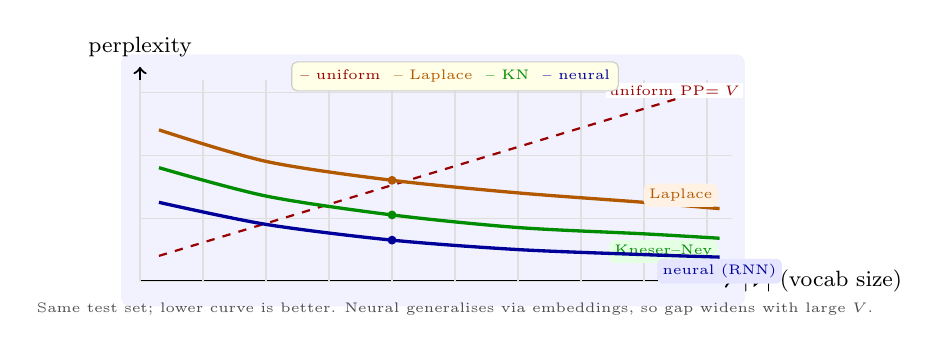
\begin{tikzpicture}[scale=0.80, font=\footnotesize]
  \fill[blue!5, rounded corners=3pt] (-0.3,-0.4) rectangle (9.6,3.6);
  \draw[->, thick] (0,0) -- (9.4,0) node[right] {$|\mathcal{V}|$ (vocab size)};
  \draw[->, thick] (0,0) -- (0,3.4) node[above] {perplexity};
  \draw[gray!25] (0,0) grid (9.4,3.2);
  % uniform baseline PP=V
  \draw[thick, red!60!black, dashed] (0.3,0.4) -- (9.2,3.1) node[pos=0.92, above, font=\tiny, fill=white, inner sep=1pt] {uniform PP$=V$};
  % Laplace (high PP)
  \draw[very thick, orange!70!black] plot[smooth] coordinates {(0.3,2.4) (2,1.9) (4,1.6) (6,1.4) (8,1.25) (9.2,1.15)} node[above left, font=\tiny, fill=orange!10, rounded corners=2pt, inner sep=2pt] {Laplace};
  % Kneser-Ney
  \draw[very thick, green!55!black] plot[smooth] coordinates {(0.3,1.8) (2,1.35) (4,1.05) (6,0.85) (8,0.75) (9.2,0.68)} node[below left, font=\tiny, fill=green!10, rounded corners=2pt, inner sep=2pt] {Kneser--Ney};
  % Neural
  \draw[very thick, blue!60!black] plot[smooth] coordinates {(0.3,1.25) (2,0.90) (4,0.65) (6,0.50) (8,0.42) (9.2,0.38)} node[below, font=\tiny, fill=blue!10, rounded corners=2pt, inner sep=2pt] {neural (RNN)};
  \fill[orange!70!black] (4,1.6) circle (2pt); \fill[green!55!black] (4,1.05) circle (2pt); \fill[blue!60!black] (4,0.65) circle (2pt);
  \node[font=\tiny, align=center, fill=yellow!10, draw=gray!40, rounded corners=2pt, inner sep=3pt] at (5.0,3.25) {\textcolor{red!60!black}{-- uniform} \ \textcolor{orange!70!black}{-- Laplace} \ \textcolor{green!55!black}{-- KN} \ \textcolor{blue!60!black}{-- neural}};
  \node[font=\tiny, text=gray!60!black] at (5.0,-0.45) {Same test set; lower curve is better. Neural generalises via embeddings, so gap widens with large $V$.};
\end{tikzpicture}
\caption{Perplexity versus vocabulary size (schematic). Uniform scales linearly. Laplace suffers most; Kneser--Ney is strong among count models; neural LMs (feedforward/RNN) achieve lowest perplexity because embeddings share statistical strength across similar histories.}
\label{fig:ppl-vocab}
\end{figure}
\section{From Scratch in Python}\label{sec:code-lm}
\begin{lstlisting}[language=Python, caption={Interpolated Kneser--Ney (bigram) and perplexity. Pure Python, no extra deps.}, label={lst:kn-ppl}]
from collections import Counter, defaultdict
import math

corpus = ["<s> the cat sat </s>", "<s> the cat ran </s>", "<s> the dog sat </s>"]
# counts
bigram_c = Counter(); unigram_c = Counter(); cont_counts = defaultdict(set)
for sent in corpus:
    toks = sent.split()
    for i, w in enumerate(toks):
        unigram_c[w] += 1
        if i > 0:
            bigram_c[(toks[i-1], w)] += 1
            cont_counts[w].add(toks[i-1])

# continuation probability
all_bigrams = len(bigram_c)
p_cont = {w: len(s)/all_bigrams for w, s in cont_counts.items()}
D = 0.75  # discount

def p_kn(prev, word):
    c_bi = bigram_c[(prev, word)]
    c_prev = unigram_c[prev]
    if c_prev == 0:
        return p_cont.get(word, 1e-8)
    # distinct continuations of prev
    uniq = sum(1 for (a, b) in bigram_c if a == prev)
    lam = D * uniq / c_prev if c_prev else 0.0
    discounted = max(c_bi - D, 0) / c_prev
    return discounted + lam * p_cont.get(word, 1e-8)

print("P_KN(sat|cat) =", round(p_kn("cat","sat"), 4))
print("P_KN(mat|cat) =", round(p_kn("cat","mat"), 4))  # unseen > 0

# perplexity of a test sentence under KN
test = "<s> the cat sat </s>".split()
log_sum = 0.0
for i in range(1, len(test)):
    p = p_kn(test[i-1], test[i])
    log_sum += math.log(p + 1e-12)  # ln
H_nats = -log_sum / (len(test)-1)
ppl = math.exp(H_nats)              # = 2^{H_bits}
print(f"Perplexity = {ppl:.2f}  (H={H_nats/math.log(2):.2f} bits)")
# compare Laplace bigram for reference
V = len(unigram_c)
def p_lap(prev, word, alpha=1.0):
    return (bigram_c[(prev, word)] + alpha) / (unigram_c[prev] + alpha*V)
print("P_Lap(mat|cat) =", round(p_lap("cat","mat"), 4))
\end{lstlisting}
Cross-entropy loss $-\log Q$ is the training objective; exponentiating it gives perplexity, so every gradient step directly lowers PP on training data (validate on held-out data to avoid overfitting).
\section{Chapter Notes}
% ============================================================
\section{Exercises}\label{sec:ch05-exercises}
\begin{enumerate}[label=E5.\arabic*, leftmargin=*, itemsep=0.7em]
    \item \textbf{MLE and zeros.} Corpus: ``\texttt{<s> a b a}'', ``\texttt{<s> a b}''. Compute $P_{\text{MLE}}(b\mid a)$, $P_{\text{MLE}}(a\mid b)$, and $P(b,a\mid\texttt{<s>})$ via the chain rule. Show that any sentence containing the unseen bigram $(b,\texttt{<s>})$ gets probability $0$ and explain why this is catastrophic for evaluation.
    \item \textbf{Laplace vs.\ Good--Turing.} With $V=10\,000$, history ``cat'' has $c(\text{cat})=1000$, $c(\text{cat,sat})=80$, $c(\text{cat,mat})=0$, and $N_{1}=4000$, $N_{2}=1500$ for bigrams. Compute $P_{\text{Lap}}(\text{sat}\mid\text{cat})$ and $P_{\text{Lap}}(\text{mat}\mid\text{cat})$ with $\alpha=1$. Then compute the Good--Turing $r^{*}$ for $r=0$ and $r=1$ and discuss which method wastes more mass on unseen bigrams.
    \item \textbf{Kneser--Ney continuation.} In a corpus, ``Francisco'' appears $100$ times but only after ``San'', while ``dog'' appears $100$ times after $80$ distinct words. With $|\{(u,v):c(u,v)>0\}|=10\,000$, compute $P_{\text{cont}}$ for each and use Eq.~\eqref{eq:kn} with $D=0.75$, $c(\text{San,Francisco})=100$, $c(\text{San})=100$, $c(\text{the,dog})=5$, $c(\text{the})=1000$ to show $P_{\text{KN}}(\text{Francisco}\mid\text{San})\gg P_{\text{KN}}(\text{Francisco}\mid\text{the})$ but $P_{\text{cont}}(\text{dog})\gg P_{\text{cont}}(\text{Francisco})$.
    \item \textbf{Neural LM and perplexity.} A feedforward LM with window $n=3$, $d=50$, $V=20\,000$, hidden $h=200$ has embedding matrix $\mathbf{E}\in\mathbb{R}^{d\times V}$ and $\mathbf{W}\in\mathbb{R}^{h\times (n-1)d}$, $\mathbf{U}\in\mathbb{R}^{V\times h}$. Count parameters. For test sentence of $N=10$ words where the model assigns $\log_{2}Q=-3$ bits each, compute $H$ and $\text{PP}=2^{H}$. If a second model gives $\text{PP}=45$, which is better and why?
    \item \textbf{Implement and compare.} Extend the Python listing to (a) compute trigram $P_{\text{KN}}$ by recursing to bigram $P_{\text{KN}}$, (b) report perplexity on a held-out sentence for Laplace vs.\ KN, and (c) replace count lookup with a tiny PyTorch feedforward NNLM ($d=16$, $h=32$) trained by cross-entropy and compare perplexities. Explain why the neural model wins on unseen $n$-grams.
\end{enumerate}
% End of Chapter 5
